% \chapter{Część techniczna/praktyczna}

% \chapter{Wymagania i narzędzia}

\chapter{[Właściwy dla kierunku -- np. Specyfikacja zewnętrzna]}
% Jeśli to Specyfikacja zewnętrzna:
% \begin{itemize}
% \item  wymagania sprzętowe i programowe
% \item  sposób instalacji
% \item  sposób aktywacji
% \item  kategorie użytkowników
% \item  sposób obsługi
% \item   administracja systemem
% \item  kwestie bezpieczeństwa
% \item  przykład działania
% \item  scenariusze korzystania z systemu (ilustrowane zrzutami z ekranu lub generowanymi dokumentami)
% \end{itemize}

\section{Wymagania sprzętowe}
\subsection{Kamera}
\quad Elementem niezbędnym do korzystania z modułu OpenLeap jest kamera, która pozwoli na pozyskanie obrazu. Rozdzielczość matrycy kamery powinna być wystarczająco duża, aby pozwolić na rozpoznanie dłoni. Nie ma tutaj minimalnych wymagań, większa rozdzielczość, czy też lepsza praca w warunkach niskiego oświetlenia kamery pozwoli na poprawniejsze działania algorytmów identyfikujących dłoń. Podobnie ma się liczba klatek na sekundę, która powinna być wystarczająco wysoka, tak aby można było sprawnie korzystać z możliwości oprogramowania. 

\subsection{Komputer}
\quad Jednostka obliczeniowa powinna zostać wyposażona w system operacyjny dający możliwość obsługi języka Python, taki warunek spełnia większość systemów operacyjnych na rynku. Komputer powinien spełniać minimalne wymagania w kwestii wydajności przetwarzania obrazu. Fakt istnienia możliwości instalacji i wykorzystania biblioteki MediaPipe przez minikomputery Raspberry Pi w wersji 3 i 4 oznacza, że wymagania nie są wysokie. 


\section{Instalacja paczki}
\quad Instalacja paczki odbywa się poprzez wykorzystanie programu \textbf{pip}, który jest instalowany automatycznie razem z językiem Python. W zależności od wybranego systemu operacyjnego komenda może przybierać różne formy, ogólnie można przyjąć poniższy zapis \ref{lst:installcom}. Komenda powinna zostać wykonane poprzez powłokę \textbf{bash} lub inną dostępną w systemie Unix-owym lub poprzez wiersz poleceń w systemie Windows. 

\begin{lstlisting}[language=bash, style=command, label={lst:installcom}, caption={Instalacja paczki}, captionpos=b]
    $ pip install openleap
\end{lstlisting}

\quad Informacje na temat biblioteki można znaleźć na platformie PyPi pod linkiem: \textbf{\href{https://pypi.org/project/openleap/}{https://pypi.org/project/openleap/}}. Na tej stronie znajduje się opis modułu, instrukcja instalacji oraz przykładowe programy i możliwości wykorzystania.

\begin{figure}[H]
    \begin{center}
        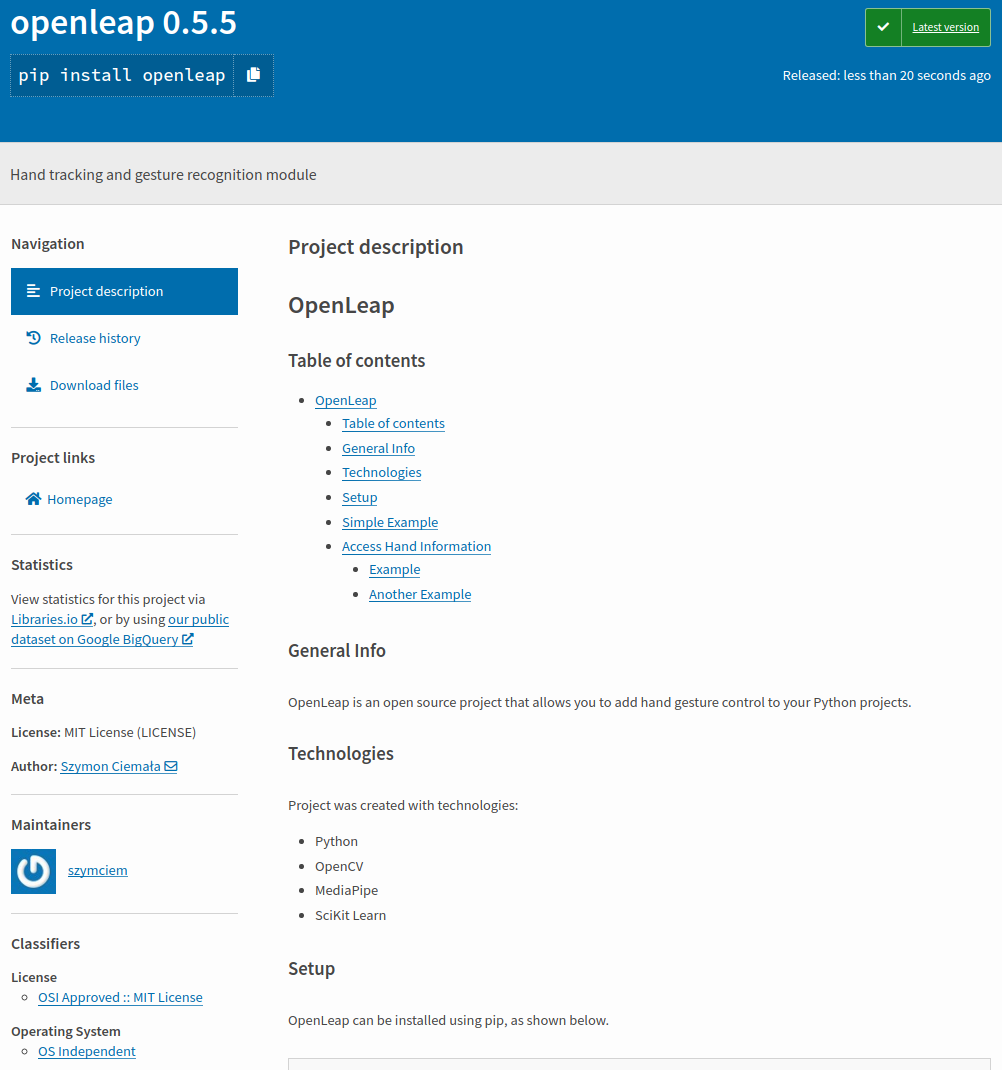
\includegraphics[width=15cm]{../images/pypi_page.png}
        \caption{Strona modułu OpenLeap na PyPi}
    \end{center}
\end{figure}

\section{Przykładowy program}

\quad Paczkę można przetestować korzystając z dostępnych funkcji klasy. Program można napisać w powłoce języka Python lub po prostu zapisać krótki program.

\begin{lstlisting}[language=python, style=programming]
    import openleap

    controller = openleap.OpenLeap(screen_show=True, 
                                   screeen_type='BLACK', 
                                   show_data_on_image=True, 
                                   gesture_model='basic')
    
    controller.loop()
\end{lstlisting}

\quad Przykładowy program pozwoli na wyświetlenie okna z widocznymi dłońmi wraz z oznaczonymi punktami charakterystycznymi oraz opisem parametrów, takich jak obrót dłoni względem nadgarstka, jej pozycja względem lewego górnego rogu obrazu kamery czy rozpoznany gest. Zrzut ekranu testowego programu znajduje się poniżej na rysunku \ref{fig:prog_screen_1}. 

\begin{figure}[H]
    \begin{center}
        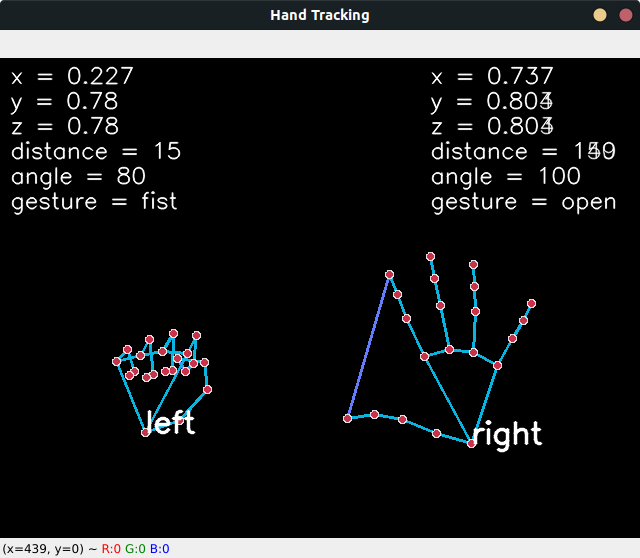
\includegraphics[width=9cm]{../images/example_program.png}
        \caption{Zrzut ekranu programu testowego}
        \label{fig:prog_screen_1}
    \end{center}
\end{figure}

\quad Dane zostają zapisane w liście składającej się z obiektów typu \textbf{dataclass}, struktura danych, która zostanie dokładnie opisana w kolejnym rozdziale, dla dłoni lewej i prawej, które przechowują wygenerowane informacje o danej dłoni. Operację pobrania danych można wykonać w poniżej przedstawiony sposób. 

\begin{lstlisting}[language=python, style=programming]
    Zbierz dane
\end{lstlisting}

\section{Funkcjonalność modułu}
\quad Paczkę można wykorzystać tam gdzie wymagane jest wykorzystanie gestów oraz ruchów dłoni. Paczka może znaleźć zastosowanie aplikacjach użytku codziennego, robotyce lub pełnić formę peryferium komputerowego.  

\subsection{Parametry}
\label{parametry}
\quad Obiekt kontrolera może zostać stworzony z wybranymi parametrami. Można wybrać czy należy wyświetlić podgląd kamery, czy wyświetlić dane na podglądzie oraz w konsoli oraz wybrać tło podglądu, czarne lub obraz z kamery. 

% \begin{itemize}
%     \item \textbf{screen\_show} - podgląd okna
%     \item \textbf{screen\_type} - typ tła: kamera ("CAM") lub czarne ("BLACK")
%     \item \textbf{show\_data\_in\_console} - wyświetlanie danych w konsoli
%     \item \textbf{show\_data\_on\_image} - wyświetlanie danych w oknie graficznym
%     \item \textbf{normalized\_position} - wyświetlanie
%     \item \textbf{gestrure\_model} - wybór modelu rozpoznającego gesty
% \end{itemize}

\begin{enumerate}
    \item \textbf{screen\_show} - podgląd okna, typ \textbf{boolean}
    \item \textbf{screen\_type} - typ tła
    \begin{enumerate}
        \item \enquote{CAM} - obraz z kamery
        \item \enquote{BLACK} - czarne tło
    \end{enumerate}
    \item \textbf{show\_data\_in\_console} - wyświetlanie danych w konsoli, typ \textbf{boolean}
    \item \textbf{show\_data\_on\_image} - wyświetlanie danych w oknie graficznym, typ \textbf{boolean}
    \item \textbf{normalized\_position} - wyświetlanie znormalizowanej pozycji, typ \textbf{boolean}
    \item \textbf{model} - wybór modelu rozpoznającego gesty
    \begin{enumerate}
        \item \enquote{basic} - gesty podstawowe
        \item \enquote{sign\_language} - język migowy
    \end{enumerate}
\end{enumerate}


\begin{figure}[H]
    \centering
    \subfloat[Obraz z kamery.]{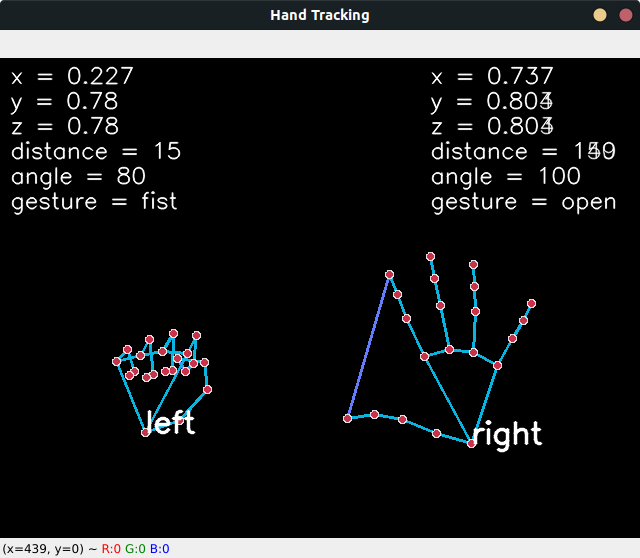
\includegraphics[width=7.3cm]{../images/example_program.png}\label{fig:f1}}
    \hfill
    \subfloat[Czarne tło.]{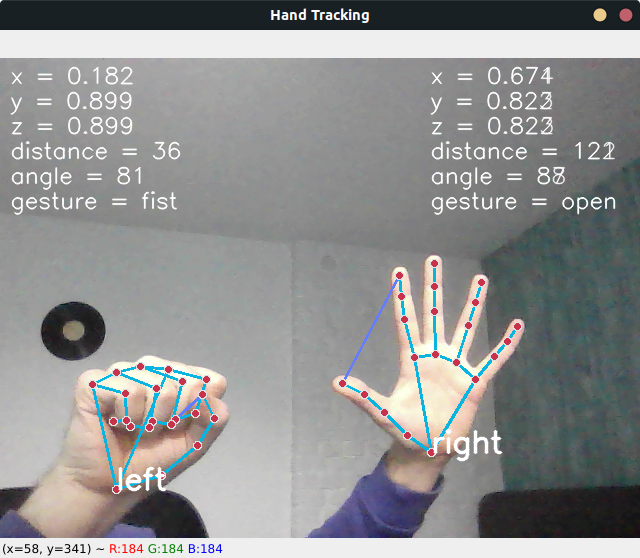
\includegraphics[width=7.3cm]{../images/cam_example.png}\label{fig:f2}}
    \caption{Parametry wyświetlanego obrazu.}
\end{figure}

\subsection{Dostępne funkcje}

\subsection{Główny wątek}
\quad Działanie kontrolera opiera się na wywoływaniu funkcji \textbf{main()}. Tą funkcję można wywołać za pomocą wybudowanej funkcji \textbf{loop()}, która po prostu wywołuje funkcję \textbf{main()} w pętli wraz z warunkiem wyjścia z programu. Takie podejście może ułatwić stosowanie kontrolera w osobnym wątku aplikacji. 
\quad Alternatywnym podejściem jest po prostu zastosowanie funkcji \textbf{main()} w pętli budowanego programu. Takie rozwiązanie daje podobny rezultat, ale bez konieczności wykorzystania osobnego wątku. 

\section{Przykłady użycia}
\subsection{Rozpoznawanie alfabetu w języku migowym}
\quad Pierwszym przykładem zastosowania jest wykorzystanie paczki do rozpoznawnia alfabetu języka migowego. Taki program może umożliwić komunikację między osobą głuchoniemą posługującą się językiem migowym, a osobą, które takiego jęzka nie zna. 


\begin{figure}[H]
    \begin{center}
        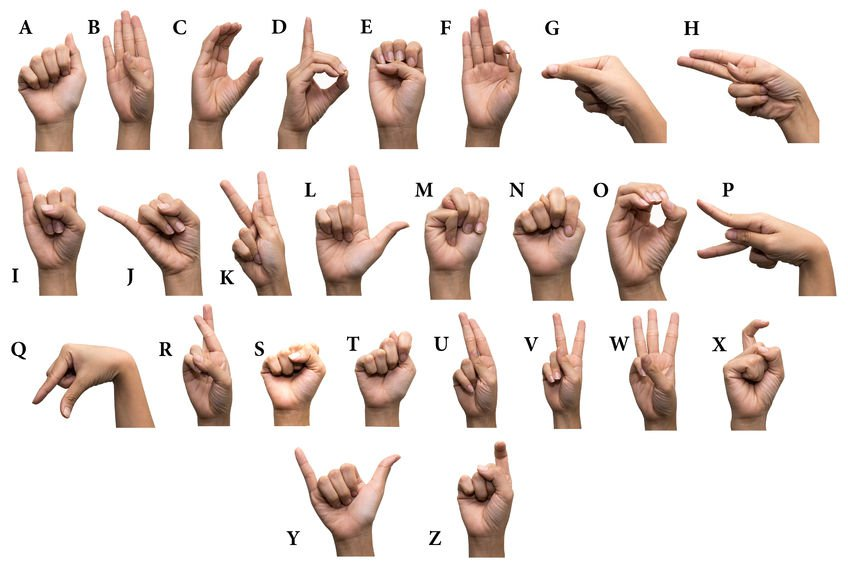
\includegraphics[width=15cm]{../images/american_sign_language.jpg}
        \caption{Gesty alfabetu języka migowego}
    \end{center}
\end{figure}

\quad Oprócz modelu rozpoznającego gesty alfabetu języka migowego, klasa została wyposażona w model rozpoznający podstawowe gesty, czyli gesty otwartej i zamkniętej dłoni. Wybór odpowiedniego modelu odbywa się w momencie tworzenia obiektu poprzez ustawienie parametru \textbf{gesture\_model}.


\begin{figure}[H]
    \centering
    \subfloat[Litery A i B.]{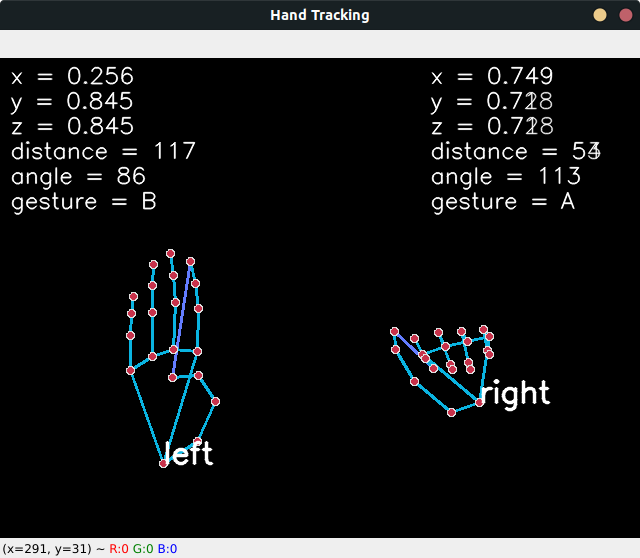
\includegraphics[width=7.3cm]{../images/a_b.png}\label{fig:f1}}
    \hfill
    \subfloat[Litery C i X.]{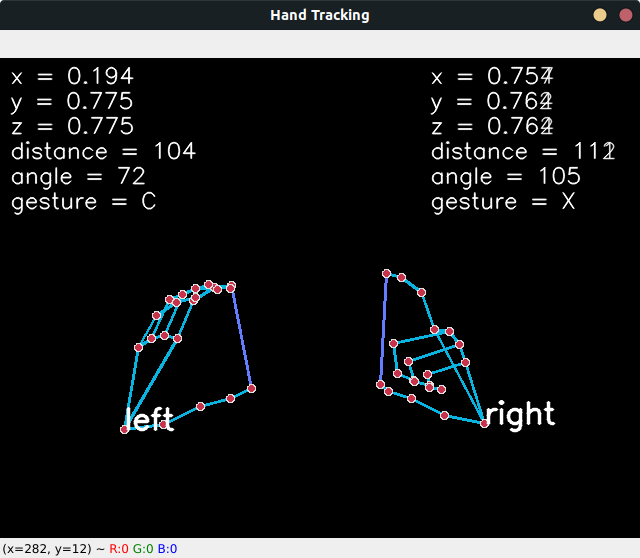
\includegraphics[width=7.3cm]{../images/c_x.png}\label{fig:f2}}
    \hfill
    \subfloat[Litery F i O.]{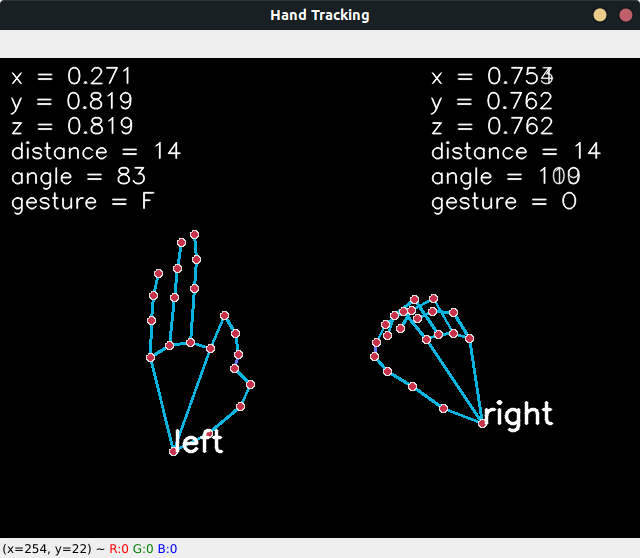
\includegraphics[width=7.3cm]{../images/f_o.png}\label{fig:f3}}
    \caption{Rozpoznawanie języka migowego .}
\end{figure}

\subsection{Interaktywny Kiosk}
\quad Kolejnym przykładem jest interktywny kiosk, który pozwala na złożenie zamówienia w sposób, który nie wymaga dotykania ekranu dotykowego. W dobie pandemii takie rozwiązanie może potencjalnie przyczynić się do spowolnienia rozprzestrzeniania się różnego rodzaju wirusów i drobnoustrojów. 


\begin{figure}[H]
    \begin{center}
        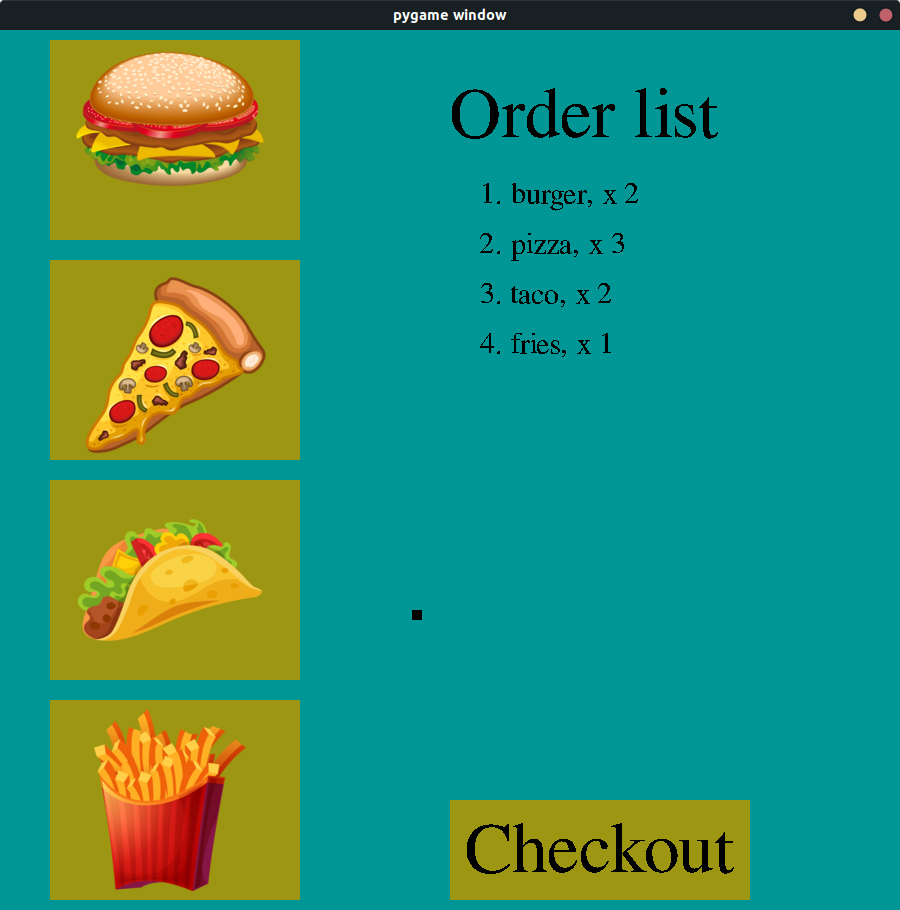
\includegraphics[width=15cm]{../images/checkout_window.png}
        \caption{Zrzut ekranu kiosku interaktywnego}
    \end{center}
\end{figure}

\quad Wskaźnik kiosku interaktywnego jest sterowany poprzez pozycję dłoni. Kliknięcie w przycisk zostaje aktywowane za pomocą wykrycia odpowiednio małej odlęgłości między końcówką palca wskazującego, a końcówką kciuka. 

\quad Odległość między tymi dwoma punktami jest obliczana automatycznie poprzez wbudowaną funkcję klasy OpenLeap. 

\subsection{Dobór koloru}
\quad Ostatnim przykładem jest wykorzystanie dłoni jako kontrolera, za którego pomocą można wybrać dowolny kolor. Takie zastosowanie może zostać wykorzystane w pracy grafika komputerowego. Dzięki temu użytkownik będzie mógł zmieniać kolor wykorzysytywanego narzędzia bez przerywania pracy, na przykład malowania. Kolor można ustawiać tyko wtedy kiedy gest lewej ręki jest gestem otwartej dłoni. 


\begin{figure}[H]
    \centering
    \subfloat[Widok dłoni.]{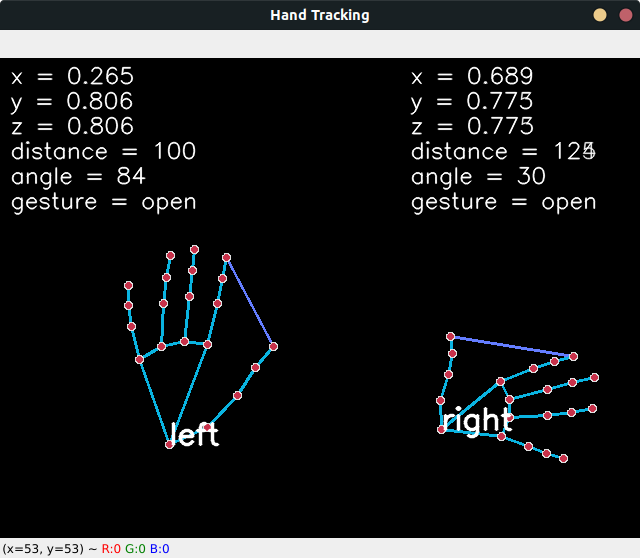
\includegraphics[width=7.3cm]{../images/yellow_hand_deg.png}\label{fig:f1}}
    \hfill
    \subfloat[Dobrany kolor.]{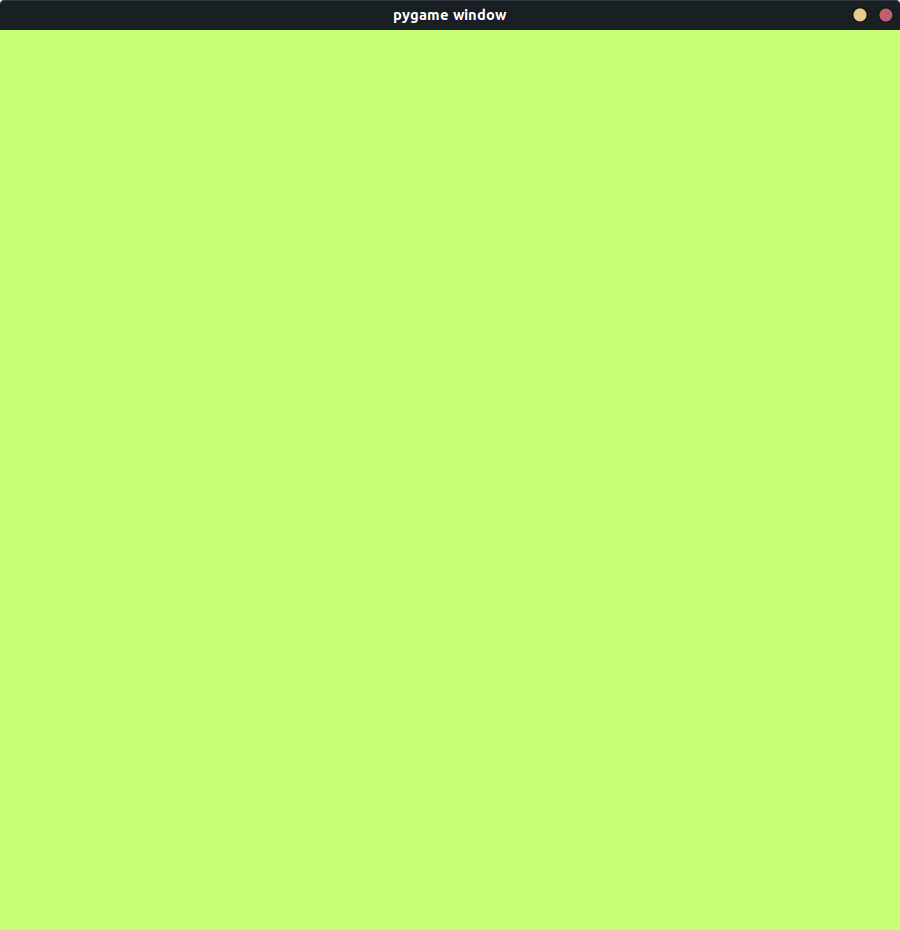
\includegraphics[width=7.3cm]{../images/yellow.png}\label{fig:f2}}
    \caption{Obrót dłoni o 30 stopni.}
\end{figure}

\begin{figure}[H]
    \centering
    \subfloat[Widok dłoni.]{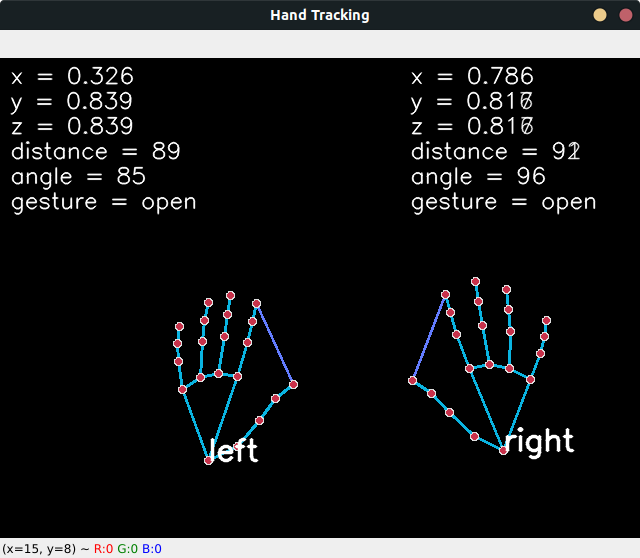
\includegraphics[width=7.3cm]{../images/blueish_hand_deg.png}\label{fig:f1}}
    \hfill
    \subfloat[Dobrany kolor.]{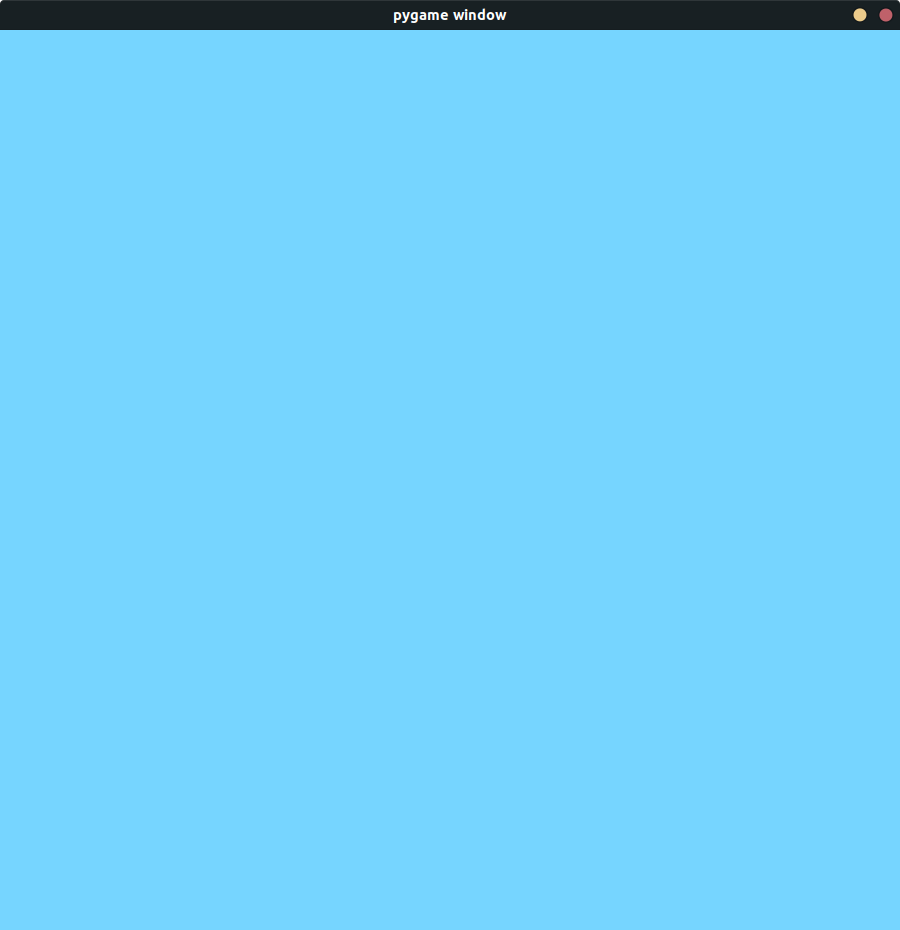
\includegraphics[width=7.3cm]{../images/blueish.png}\label{fig:f2}}
    \caption{Obrót dłoni o 96 stopni.}
\end{figure}

\begin{figure}[H]
    \centering
    \subfloat[Widok dłoni.]{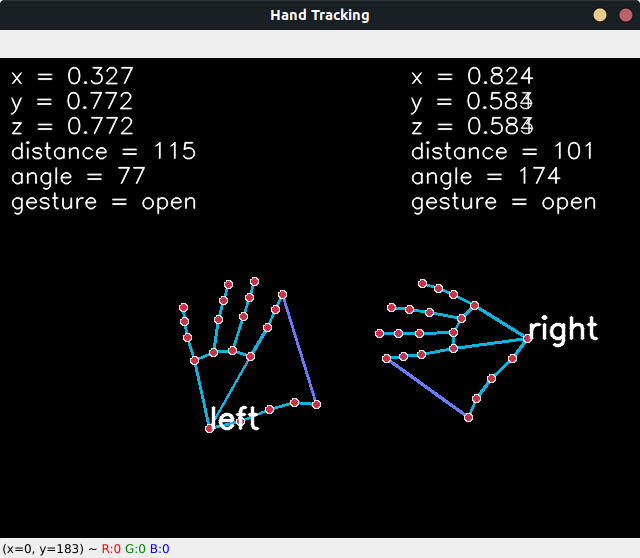
\includegraphics[width=7.3cm]{../images/pink_hand_deg.png}\label{fig:f1}}
    \hfill
    \subfloat[Dobrany kolor.]{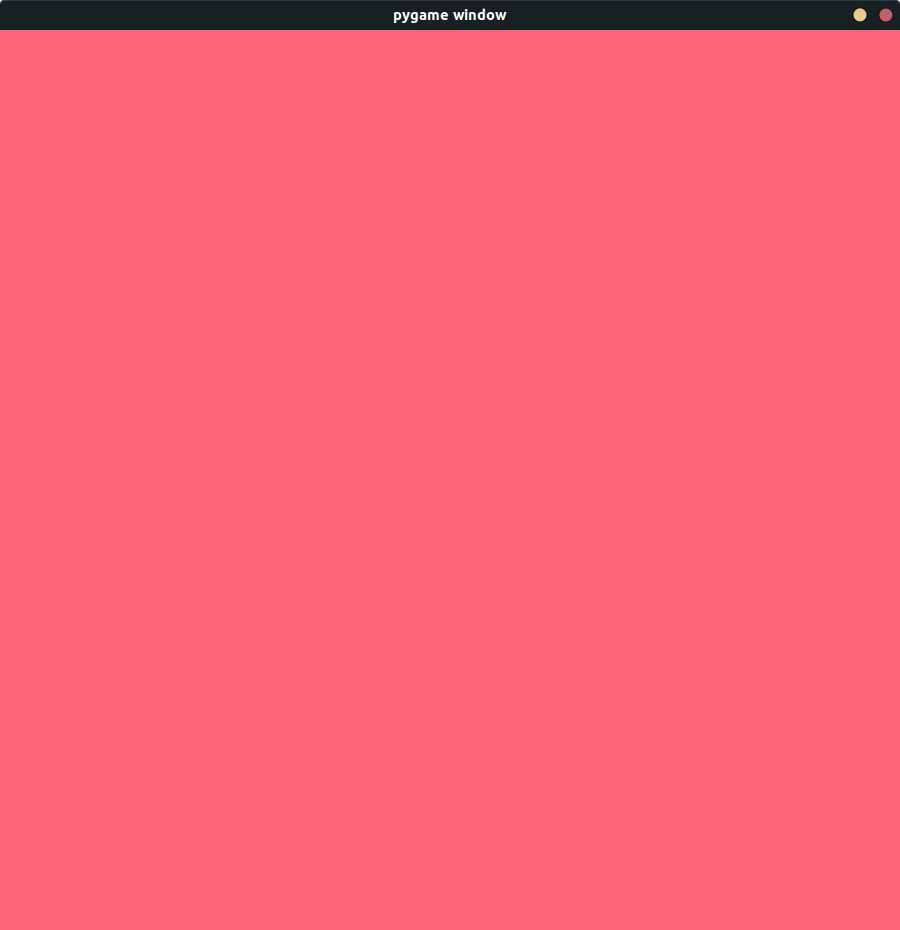
\includegraphics[width=7.3cm]{../images/pink.png}\label{fig:f2}}
    \caption{Obrót dłoni o 174 stopni.}
\end{figure}

\quad Dodatkową opcją jest ustawienie saturacji poprzez obliczenie jej wartości na podstawie odległości między palcem wskazującym, a kciukiem. 

\begin{figure}[H]
    \centering
    \subfloat[Widok dłoni.]{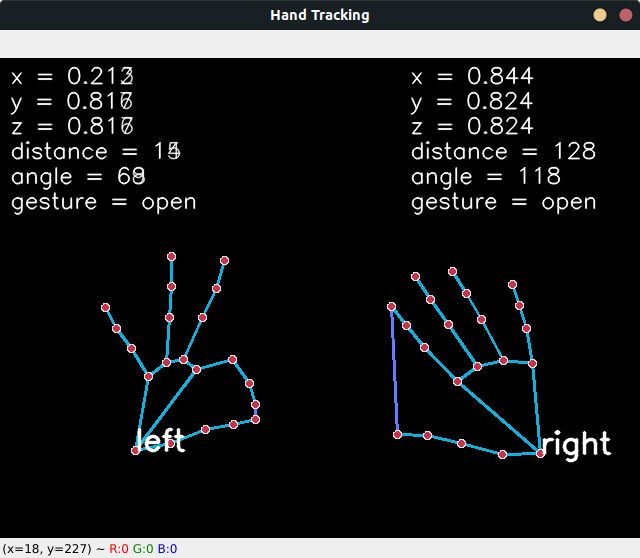
\includegraphics[width=7.3cm]{../images/zero_sat_hand_deg.png}\label{fig:f1}}
    \hfill
    \subfloat[Dobrany kolor.]{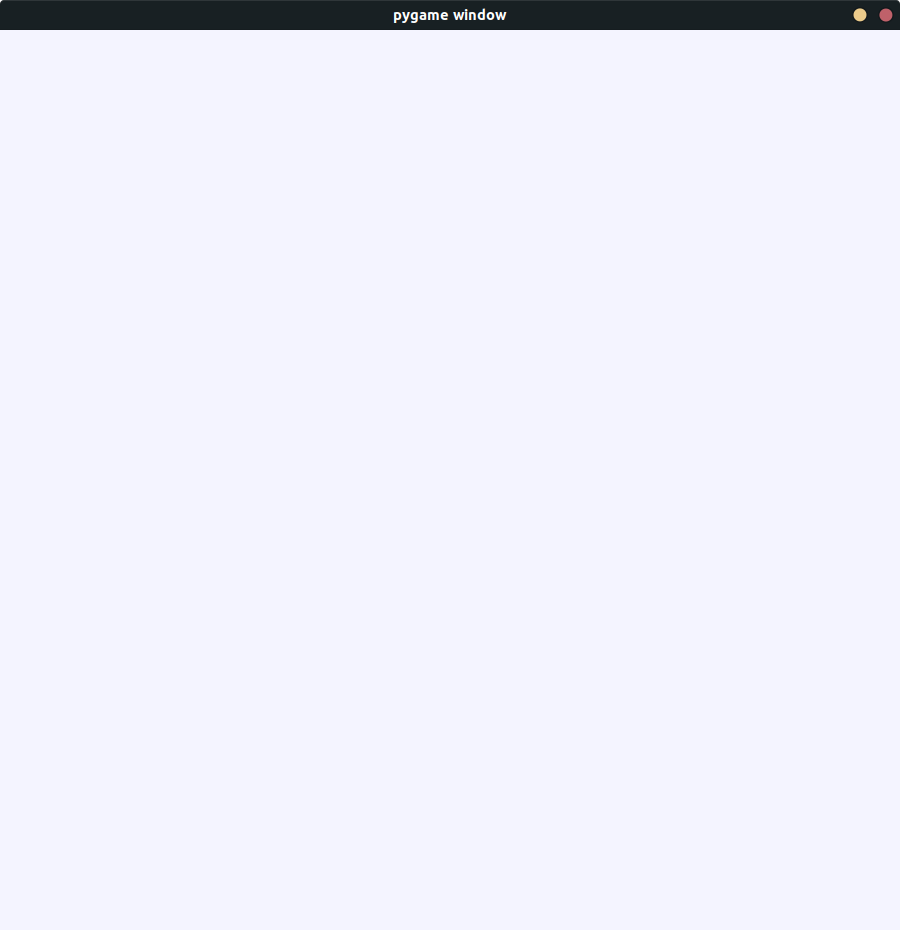
\includegraphics[width=7.3cm]{../images/zero_sat.png}\label{fig:f2}}
    \caption{Ustawienie saturacji}
\end{figure}


\quad Podobnie jak obliczenie odległości między palcami, biblioteka oblicza obrót dłoni wokół osi Z punktu opisującego pozycję nadgarstka.


\section{Stworzenie nowego modelu}

\quad Użtkownik biblioteki może stworzyć własny model rozpoznający gesty. Wykorzystać do tego można program napisany przy pomocy Jupyter Notebook. Plik jest dostępny na platformie \href{https://github.com/szymciem8/OpenLeap/blob/main/Jupyter%20Notebook/Create%20your%20own%20model/Gesture%20Detection.ipynb}{\textbf{GitHub}}. Plik posiada rozszerzenie \textbf{.ipynb}.

\quad Dokładny opis tworzenia modelu zostanie opisany w kolejnym rozdziale dotyczącym specyfikacji wewnętrznej. 